\section{Symmetric Matrices}
%Lecture Sep 18
\begin{definition}[Set of symmetric matrices]
The set of $n$ by $n$ square matrices is defined as
$$S^n = \{A\in \reals^{n\times n} | A = A^{\trans} \}$$
\end{definition}



In the following, we give a few examples of symmetric matrices.

\begin{example}[Hessian matrix]
A Hessian matrix of a function $F:\reals^n\to \reals$ is a matrix that each element is the 2nd order partial derivative of $F$, i.e.,
$$[\nabla^2 F]_{ij} = \frac{\partial^2 F(x)}{\partial x_i \partial x_j}$$
\end{example}

\begin{example}[Quadratic function] Let $q: \reals^n \rightarrow \reals$ be a quadratic function, that is,
\begin{align*}
q(x) &= \sum^n_{i=1}\sum^n_{j=1}a_{ij}x_ix_j + \sum^n_{i=1}c_ix_i + d\\
&= x^{\trans}Ax + c^{\trans}x + d\\
&= \frac{1}{2}x^{\trans}(A + A^{\trans})x + c^{\trans}x + d\\
&= \frac{1}{2}
\begin{bmatrix}%
x^{\trans}& 1
\end{bmatrix}
\begin{bmatrix}%
A + A^{\trans} & c\\
c^{\trans} & 2d
\end{bmatrix}
\begin{bmatrix}%
x\\
1
\end{bmatrix}
\end{align*}

The third equality is obtained by realizing that $A$ must be a symmetric matrix here, so $A + A^{\trans} = A + A=2A$.


(1) Let
\begin{align*}
q_1(x) &= x^{\trans}Ax = \sum_{i=1}\sum_{j=1}a_{ij}x_ix_j\\
&= a_{11}x_1^2 + a_{12}x_1x_2 + \cdots + a_{21}x_2x_1 +\cdots
\end{align*}

\begin{align*}
\frac{d}{dx_k}q_1(x) &= \frac{d}{dx_k}\left(a_{kk}x_k^2 + \sum_{l\neq k}x_lx_k(a_{lk}+a_{kl})\right)\\
&= (a_{kk} + a_{kk})x_k + \sum_{l\neq k}x_l(a_{lk} + a_{kl}) \\
&= \sum^n_{i=1}(a_{lk} + a_{kl})x_l\\
&= \sum^n_{i=1}\left([A]_{kl} + [A]_{lk}\right)x_l
\end{align*}

Hence,
\begin{align*}
\nabla q_1(x) &= (A + A^{\trans})x\\
\left[\nabla^2 q_1(x)\right]_{kj} &= \frac{d}{dx_j}\left(\frac{d}{d x_k}q_1(x)\right)\\
&= [A]_{kj} + [A]_{jk}\\
\nabla^2 q_1(x) &= A + A^{\trans}
\end{align*}

(2) Let $q_2(x) = c^{\trans}x = \sum^n_{i=1}c_ix_i$,
\begin{align*}
\frac{d}{dx_k} q_2(x) &= \frac{d}{dx_k}\left(\sum^n_{i=1}c_ix_i\right) = c_k\\
\nabla q_2(x) &= 
\begin{bmatrix}%
\frac{\partial q_2(x)}{\partial x_1}\\
\vdots\\
\frac{\partial q_2(x)}{\partial x_n}
\end{bmatrix}=
\begin{bmatrix}%
c_1\\
\vdots\\
c_n
\end{bmatrix} = c
\end{align*}

Combine (1) and (2), and because $q(x) = x^{\trans}Ax + c^{\trans}x + d$, we take Taylor approximation of $q(x)$ up to the second order:
\begin{align*}
\tilde{q}(x) &= q(0) + \nabla q(0)^{\trans}x + \frac{1}{2}x^{\trans}\nabla^2q(0)x\\
&= d + c^{\trans}x + \frac{1}{2}x^{\trans}(A + A^{\trans})x
\end{align*}

\end{example}


\section{Symmetric Matrices and Eigenvectors}

\begin{theorem}{4.18 \& 4.2 in textbook}
	
	For any matrix in $S^n = \{A\in \reals^{n\times n} | A = A^{\trans} \}$, we have
	
	1) All eigenvalues are purely real(so eigenvectors can be picked purely real).
	
	2) $GM(\lambda_i) = AM(\lambda_i)$: Symmetric matrix is always diagonalizable.
	
	3) Eigenvectors of distinct eigenvalues are $\perp$, i.e.,
	
\qquad $\xi_{\lambda_i} = N(A - \lambda_iI)\perp \xi_{\lambda_j} = N(A - \lambda_jI)$, where $\xi_{\lambda_i}$ denotes the eigenspace w.r.t eigenvalue $\lambda_i$ (also, it is the null space of matrix $(A - \lambda_iI)$).
\end{theorem}

Implication: We can pick the basis for each eigenspace to be an orthogonal basis(e.g, pick the eigenvectors of this symmetric matrix), because we have "full set" of eigenvectors($n$ linearly independent vectors) and we can always write:\\


\begin{theorem} [Spectral Decomposition] For an $n$ by $n$ symmetric matrix $A$, we always have the following spectral decomposition
\begin{align*}
A &= U\Lambda U^{-1}\\
&= U\Lambda U^{T}\\
&= 
\begin{bmatrix}
u^{(1)} & u^{(2)} & \cdots & u^{(n)}\\
\end{bmatrix}
\begin{bmatrix}
\lambda_1 & 0 & 0\\
0 & \ddots & 0\\
0 & 0 & \lambda_n
\end{bmatrix}
\begin{bmatrix}
u^{(1)^{\trans}}\\
\vdots\\
u^{(n)^{\trans}}
\end{bmatrix}\\
&= \sum^n_{i=1}\lambda_iu^{(i)}u^{(i)^{\trans}}
\end{align*}

\end{theorem}
To summarize, an $n$ by $n$ matrix $A$ is diagonalizable iff there are $n$ linearly independent eigenvectors(subject to scaling factors). Furthermore, if $A$ is diagonalizable, that is, $A = U\Lambda U^{-1}$, then $\Lambda$ is diagonal matrix with all its entries are the eigenvalues and $U$ is a collection of all its eigenvectors. 



\section{Variational Characterization of eigenvalues of symmetric matrix} 

Let's consider an $n$ by $n$ symmetric matrix $A$, we arrange the eigenvalues of $A$ in a decreasing order, i.e.,
$$\lambda_{max}(A) = \lambda_1 \geq \lambda_2 \geq \cdots \geq \lambda_n =\lambda_{min}(A)$$

\begin{definition}[Rayleigh quotient] Let $A=A^*$ be a $n$ by $n$ a self-joint matrix, the Rayleigh quotient is defined as 
$$R(x)= \frac{x^{\trans}Ax}{x^{\trans}x}\quad  \forall x\neq 0$$
\end{definition}


\begin{theorem}
For $A\in S^n$, we have 
$$\lambda_{min}(A) \leq \frac{x^{\trans}Ax}{\Vert x\Vert^2}\leq \lambda_{max}(A),\quad \forall x \neq 0$$
\end{theorem}


\begin{proof}
	\begin{align*}
	x^{\trans}Ax &= x^{\trans}U\Lambda U^{\trans}x\\
	&= \bar{x}^{\trans}\Lambda\bar{x}\\
	&= \sum^n_{i=1}(\bar{x}_i)^2\lambda_i\\
	&\leq \sum^n_{i=1}(\bar{x}_i)^2\lambda_{max}(A)\\
	&= \Vert\bar{x}\Vert^2\lambda_{max}(A)
	\end{align*}
where $\bar{x}=U^{\trans}x$, and note that $\Vert \bar{x}\Vert = \Vert {x}\Vert$ since $U$ is orthogonal. Use similar trick we could obtain the lower bound for $x^{\trans}Ax$. By a simple rearrangement we yield the desired result
	\begin{equation*}
	\lambda(A)_{min}\Vert\bar{x}\Vert^2 \leq x^{\trans}Ax \leq \Vert\bar{x}\Vert^2\lambda_{max}(A)
	\end{equation*}
	
	\begin{equation*}
	\lambda(A)_{min} \leq \frac{x^{\trans}Ax}{\Vert\bar{x}\Vert^2} \leq \lambda_{max}(A)
	\end{equation*}
\end{proof}


\subsection{Positive (Semi) Definite matrices (PD and PSD)}

\begin{definition}

	A symmetric matrix $A\in S^n$ is positive semi-definite definite(PSD) if $x^{\trans}Ax \geq 0$, $\forall x\in \reals^n$ and $x\neq 0$.

	Furthermore, a symmetric matrix $A\in S^n$ is positive definite(PD) if $x^{\trans}Ax > 0$, $\forall x\in \reals^n$ and $x\neq 0$.

\end{definition}

Also, we usually denote the set of PSD matrix and the set of PD matrix as
$$PSD: S^n_{+} = \{A\in S^n \vert A\succeq 0\}$$
$$PD: S^n_{++} = \{A\in S^n \vert A\succ 0\}$$

Note: The curled inequality symbol $\succeq$ (and its strict form $\succ$) is used to denote generalized inequality: between vectors, it represents component-wise inequality; between matrices, it represents matrix inequality. We will give an introduction regarding this in later chapter.

\begin{theorem}[Necessary and sufficient conditions for PSD and PD]

(1) A symmetric matrix is PSD iff all its eigenvalues $\geq 0$, or, all its \textbf{principal minors} are non-negative.

(2) A symmetric matrix is PD iff all its eigenvalues $> 0$, or, all its \textbf{leading principal minors} are positive (Sylvester's criterion).
\end{theorem}

\begin{proof}
	First, assume $A\in S^n$ is PD, we will show that all $\lambda_i > 0$. 
	
	\begin{equation*}
	x^{\trans}Ax = x^{\trans}U\Lambda U^{\trans}x = \bar{x}^{\trans}\Lambda\bar{x} = \sum^n_{i=1}\lambda_i(\bar{x}_i)^2 >0
	\end{equation*}
	Since $A$ is PD and $x\neq 0$, and it is always diagonalizable for a symmetric matrix.
	
	Since the choice of $x$ is arbitrary, to show this implies $\lambda_j > 0, \forall j\in [n]$, we set:
	$$\bar{x} = e_j = 
	\left[
	\begin{matrix}
	0\\
	\vdots\\
	0\\
	1\\
	0\\
	\vdots\\
	0\\
	\end{matrix}
	\right]
	$$
	where only the $j$th entry is 1.
	$$0 < U^{(j)^{\trans}} U\Lambda U^{\trans}U^{(j)} =e_j^{\trans}\Lambda e_j = \lambda_j$$
	
	And now we assume all eigenvalues are positive, and we want to show that $A$ is PD:
	$$x^{\trans}Ax =x^{\trans}U\Lambda U^{\trans}x = \bar{x}^{\trans}\Lambda \bar{x} = \sum^n_{i=1}(\bar{x}_i)^2\lambda_i > 0$$
	
	The proof for PSD case is similar, simply replacing the strict inequalities with inequalities.
\end{proof}


Recall some previous results and note that, for $A\in S^n$,

(1) $\det(A) = \prod^n_{i=1}\lambda_i$

(2) $\det(A) = 0$ iff there exist eigenvalue $\lambda_i = 0$:

(3) Combine (1) and (2) and our proof above, we have

\qquad $\rightarrow$ PD matrices are invertible

\qquad $\rightarrow$ PSD matrices are invertible only if they are also PD (i.e., no zero eigenvalues)



\subsection{Ellipses} 

An ellipse can be defined geometrically as a set or locus of points in the Euclidean plane. Let's consider the following set(an ellipse)
$$
\xi = \{x\in \reals^n \vert (x - x^{(0)})^{\trans} P^{-1}(x - x^{(0)}) \leq 1 \}
$$
where matrix $P$ is PD.

\begin{marginfigure}
	\centering
	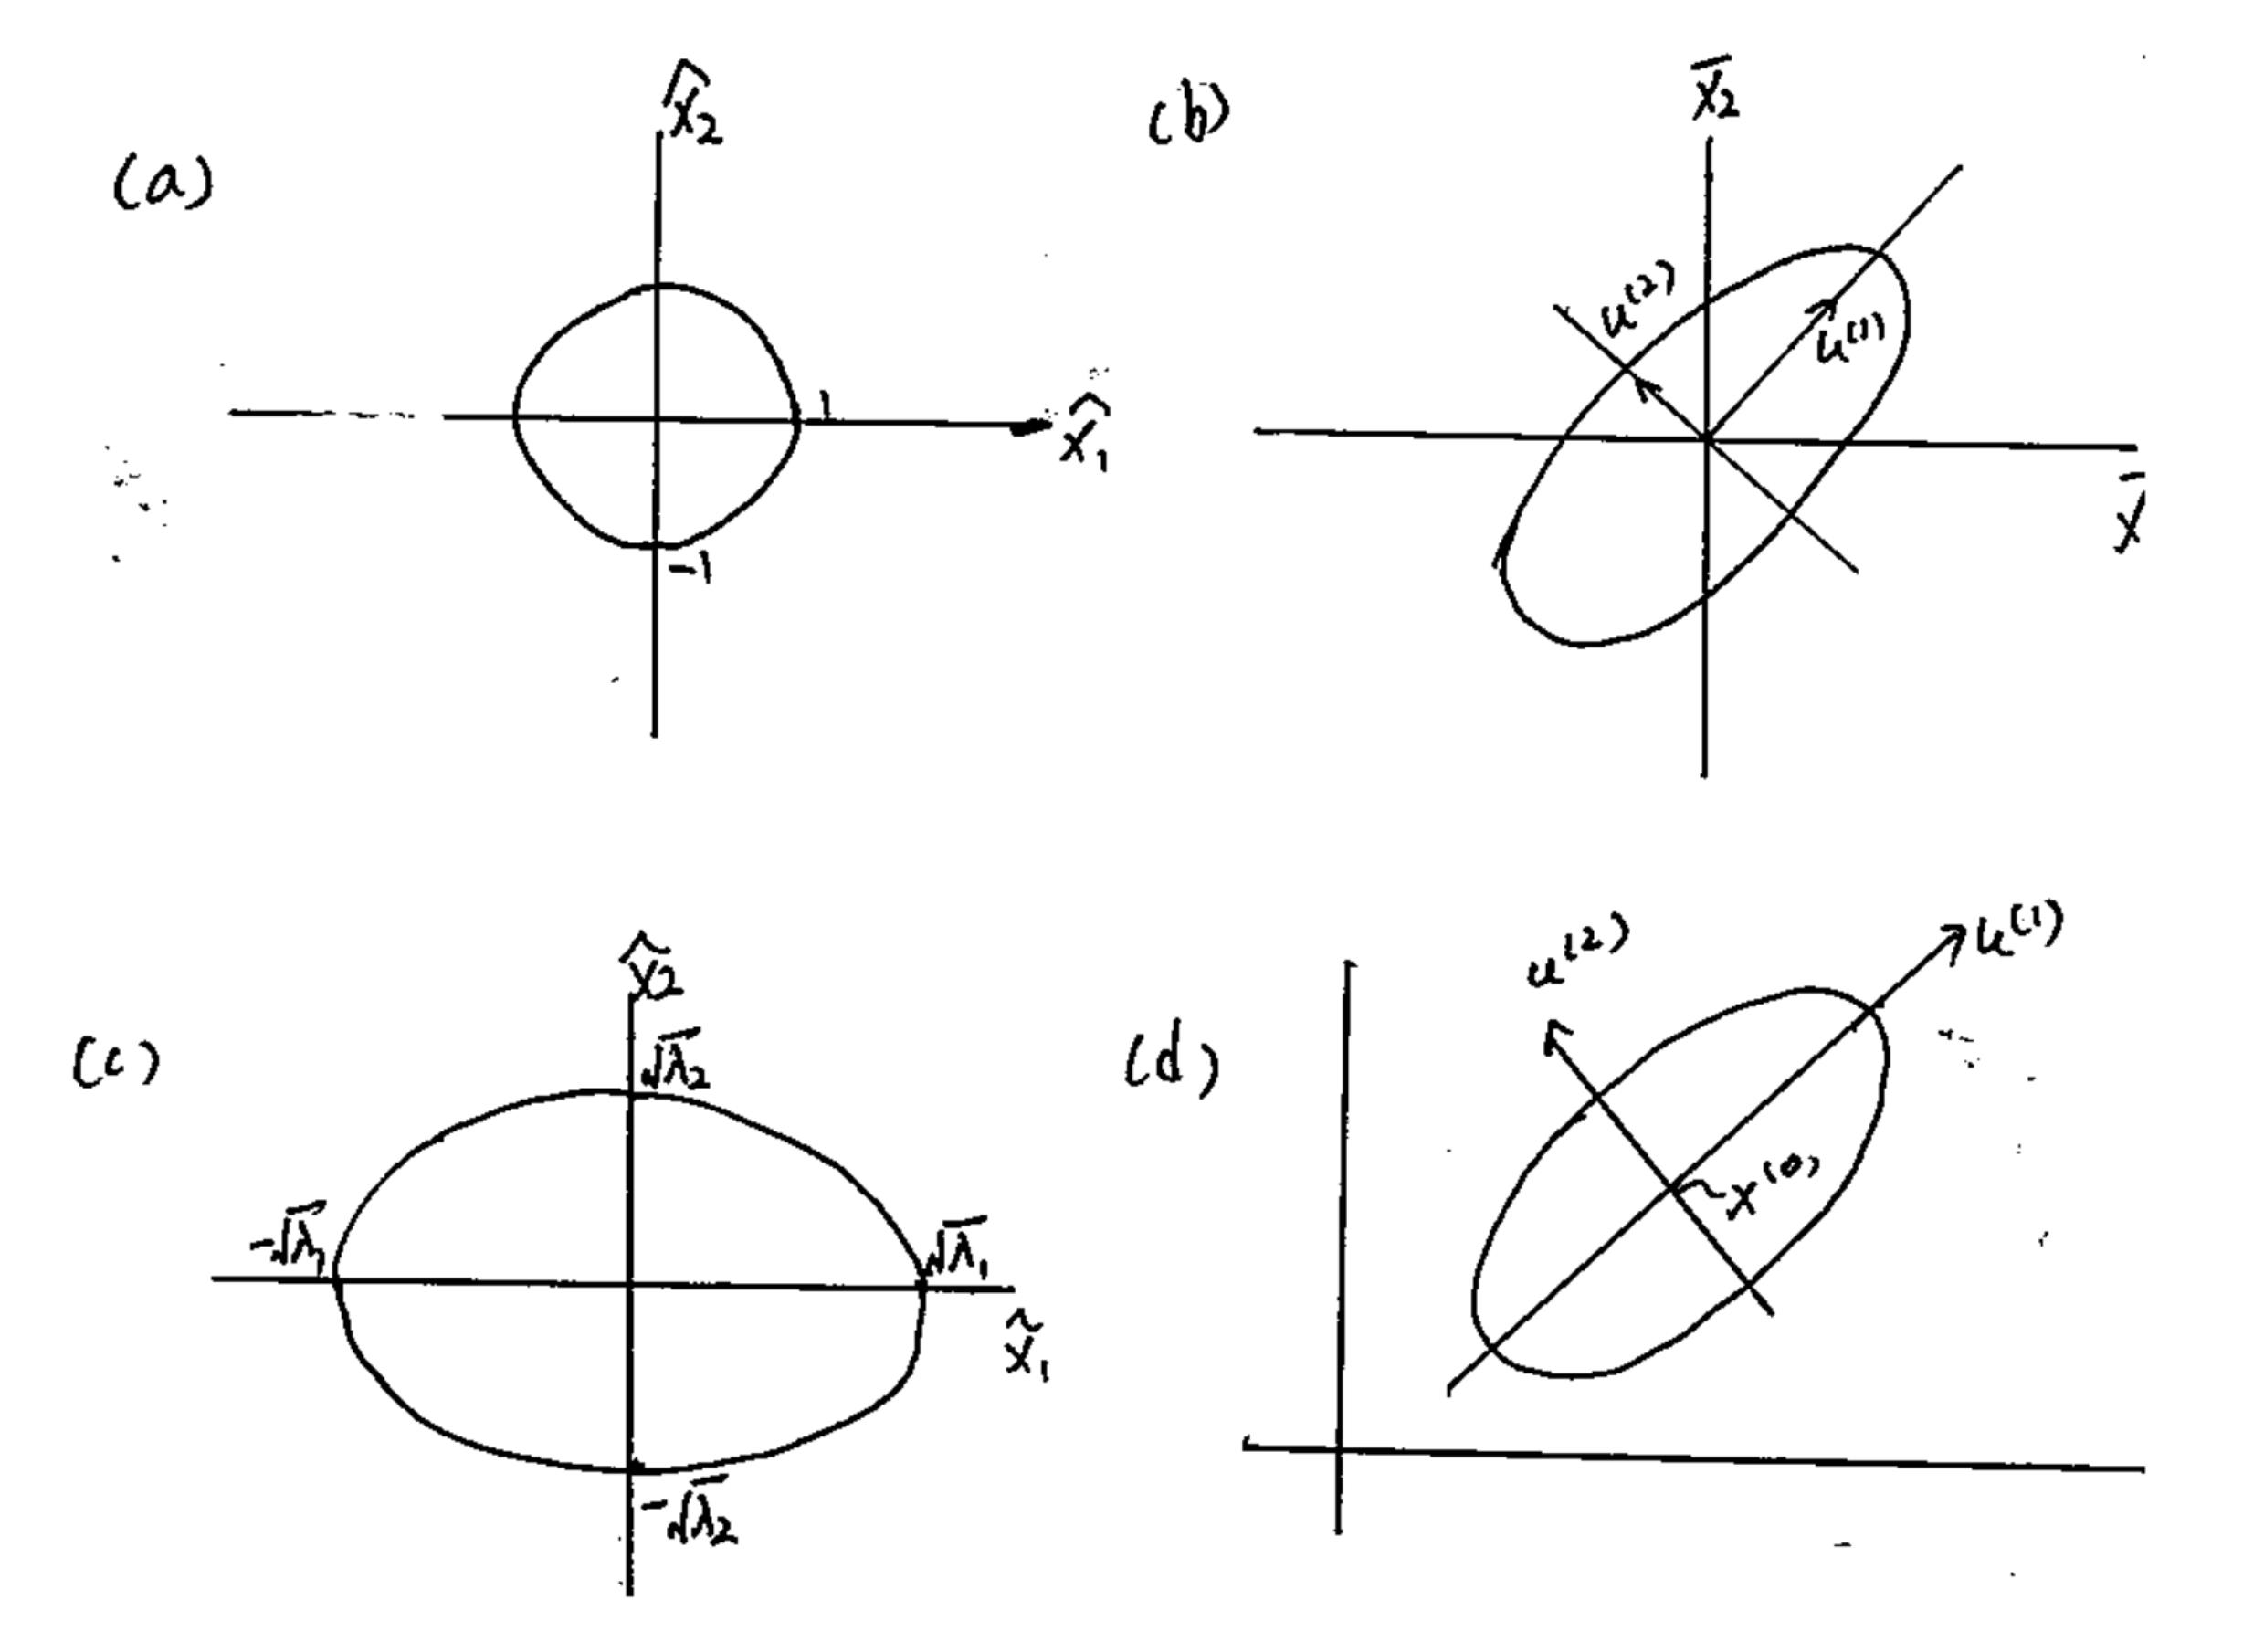
\includegraphics[width=2.1in,height=2.1in]{figures/ch03/figure2.jpg}
	%\caption{This is an inserted JPG graphic} 
	%\label{fig:graph} 
\end{marginfigure}

Note that the argument above is a quadratic function:
\begin{align*}
(x - x^{(0)})^{\trans}P^{-1}(x - x^{(0)}) &= x^{\trans}P^{-1}x - 2x^{(0)^{\trans}}P^{-1}x + x^{(0)^{\trans}}P^{-1}x^{(0)}\\
&= x^{\trans}Ax + c^{\trans}x + d
\end{align*}

Let's look at the set $\xi$, clearly it is centered at $x = x^{(0)}$, and we further simplify it by defining $\bar{x}=x-x^{(0)}$
\begin{align*}
1 &\geq (x - x^{(0)})^{\trans}P^{-1}(x - x^{(0)})\\
&= \bar{x}^{\trans}P^{-1}\bar{x}\\
&= \bar{x}^{\trans}(U\Lambda U^{\trans})^{-1}\bar{x}\\
&= \bar{x}^{\trans}(U^{\trans})^{-1}\Lambda^{-1}U^{-1}\bar{x}\\
&= \bar{x}^{\trans}U\Lambda^{-1}U^{\trans}\bar{x}\\
&= \tilde{x}^{\trans}\Lambda^{-1}\tilde{x}\\
&= \sum^n_{i=1}(\frac{\tilde{x_i}}{\sqrt{\lambda_i}})^2\\
&= \sum^n_{i=1}(\hat{x}_i)^2\\
&= \Vert \hat{x}\Vert^2
\end{align*}



\vspace{0.3cm}
Following are some examples of where symmetric and PSD matrix are important.

\begin{example}[Sample variance and PSD matrices] Given the dataset $x^{(1)}, x^{(2)}, ..., x^{(m)}$ all $x^{(i)}\in \reals^n$, recall that

Sample mean: $\mu = \frac{1}{m}\sum^m_{i=1}x^{(i)}$

Sample covariance: $\Sigma = \frac{1}{m}\sum^m_{i=1}(x^{(i)}-\mu)(x^{(i)}-\mu)^{\trans}$, where $(x^{(i)}-\mu)(x^{(i)}-\mu)^{\trans}$ is the outer-product of centered data points.

Let's consider an example with $m=3$:

$$x^{(1)} =
\left[
\begin{matrix}
1\\
2
\end{matrix}
\right]x^{(2)} =
\left[
\begin{matrix}
4\\
4
\end{matrix}
\right]x^{(3)} =
\left[
\begin{matrix}
4\\
0
\end{matrix}
\right]\mu =
\left[
\begin{matrix}
3\\
2
\end{matrix}
\right]\tilde{x}^{(1)} =
\left[
\begin{matrix}
-2\\
0
\end{matrix}
\right]\tilde{x}^{(2)} =
\left[
\begin{matrix}
1\\
2
\end{matrix}
\right]\tilde{x}^{(3)} =
\left[
\begin{matrix}
1\\
-2
\end{matrix}
\right]
$$
where we take $\tilde{x}^{(i)}=x^{(i)}-\mu$, and $\mu$ is the sample mean.

So we could compute the covariance matrix by
\begin{align*}
\Sigma &= \frac{1}{3} \left(\tilde{x}^{(1)}\tilde{x}^{(1)\trans}+\tilde{x}^{(2)}\tilde{x}^{(2)\trans}    +\tilde{x}^{(3)}\tilde{x}^{(3)\trans}\right)\\
&= \left[
\begin{matrix}
2&0\\
0&\frac{8}{3}
\end{matrix}
\right]
\end{align*}

It could be easily verified that the quadratic function $(x - \mu)^{\trans} \Sigma^{-1}(x - \mu)$ could be visualize as an ellipses with the choice $\gamma$ = 2, i.e., the set $\xi_{\gamma} = \{x | (x - \mu)^{\trans} \Sigma^{-1}(x - \mu)\leq \gamma \}$ is an ellipses.


To prove $\Sigma\geq 0$, let's consider sample variance of the scalar product for $i\in [m]$ with choice $\Vert w\Vert=1$
$$S^{(i)} =w^{\trans}x^{(i)} =\langle w, x^{(i)}\rangle$$

sample mean:
$$\tilde{S} = \frac{1}{m}\sum^m_{i=1}s^{(i)} = \frac{1}{m}\sum^m_{i=1}w^{\trans}x^{(1)} = w^{\trans}\mu$$

sample variance: 
\begin{align*}
\sigma^2 &= \frac{1}{m}\sum^m_{i=1}(s^{(i)} - w^{\trans}\mu)^2 \\
&= \frac{1}{m}\sum^m_{i=1}(w^{\trans}(x^{(i)} -\mu))^2\\
&=\frac{1}{m}\sum^m_{i=1}w^{\trans}(x^{(i)}-\mu)(x^{(i)}-\mu)^{\trans}w\\
&= w^{\trans}[\frac{1}{m}\sum^m_{i=1}(x^{(i)}-\mu)(x^{(i)}-\mu)^{\trans}]w\\
&= w^{\trans}\sum w
\end{align*}

Hence it is obviously non negative(so it is PSD) for any choice of $w$. The proof is completed.
\end{example}

\section{Square-root matrix and Cholesky decomposition}

From previous results(spectral decomposition), any PSD(and certainly for any PD) matrix can be written as
\begin{align*}
A &= U\Lambda U^{\trans} \\
&=U\Lambda^{\frac{1}{2}}\Lambda^{\frac{1}{2}}U^{T}\\
&= U\Lambda^{\frac{1}{2}}U^{\trans}U\Lambda^{\frac{1}{2}}U^{\trans}
\end{align*}
where $\Lambda^{\frac{1}{2}}=
\begin{bmatrix}%
	\sqrt{\lambda_1}& & \\
	 &\ddots& \\
	 & &\sqrt{\lambda_n}
\end{bmatrix}$,
and the third equality is due to $U^{\trans}U=I$ ($U$ is orthogonal and so $U^{-1}=U^{\trans}$).


The quantity $A^{\frac{1}{2}} = U\Lambda^{\frac{1}{2}}U^{\trans}$ is called the square root matrix of $A$, and furthermore, $A$ is PSD(PD) iff there exists a unique $A^{\frac{1}{2}}$ is a PSD(PD) matrix.

Now, let's see how to obtain the Cholesky decomposition. We rewrite the matrix decomposition as
\begin{align*}
A &= U\Lambda U^{\trans} \\
&=U\Lambda^{\frac{1}{2}}\Lambda^{\frac{1}{2}}U^{T}\\
&= U\Lambda^{\frac{1}{2}}U^{\trans}U\Lambda^{\frac{1}{2}}U^{\trans}\\
&=\beta^{\trans}\beta\\
&=(QR)^{\trans}QR\\
&=R^{\trans}Q^{\trans}QR\\
&=R^{\trans}R
\end{align*}

where we let $\beta=\Lambda^{\frac{1}{2}}U^{\trans}$, and apply QR decomposition on this square matrix $\beta$(recall that it is unique to any square matrix). Finally, we express matrix $A$ as a product of triangular matrices, where $R^{\trans}$ is lower triangular and $R$ is upper triangular.



